\section*{Supporting Asset Identification \& Valuation}
\addcontentsline{toc}{section}{Supporting Asset Identification \& Valuation}

In figure \ref{fig:impact2} the impact assessment is reported.

As we can see from the assessment, the potential compromises with higher overall impact are the ones tied to the integrity of the services of \texttt{Software distribution}, \texttt{Diginetwerk} \texttt{routing\&communication}, and \texttt{Result computation}. Also, we can observe that the impact on personnel, the economy, and the environment is estimated to be 1. 

Instead of just using the maximum of impacts, the overall impact is computed by applying a weighted average of capacity, performance, branding, and regulatory. Since the branding impact is almost always high (except for third-party incidents) because the election is an event of national matter, and because we believe that capacity and performance has higher priority, we put higher weight 1 on the latter, and 0.5 on the first two indexes.

In figure \ref{fig:linkage} the linkage between the primary and supporting assets can be observed. For example, we found that the process of inputting the ballots data has the following supporting assets

\begin{itemize}
    \item \texttt{Input Officials}
    \item \texttt{Diginetwerk}
    \item \texttt{Virtual Desktop Infrastructure (Citrix)}
    \item \texttt{DHV Software}
    \item \texttt{GSB PCs}
    \item \texttt{Secure Store for GSB PCs}
\end{itemize}


\newpage

\begin{figure}[h!]
    \centering
    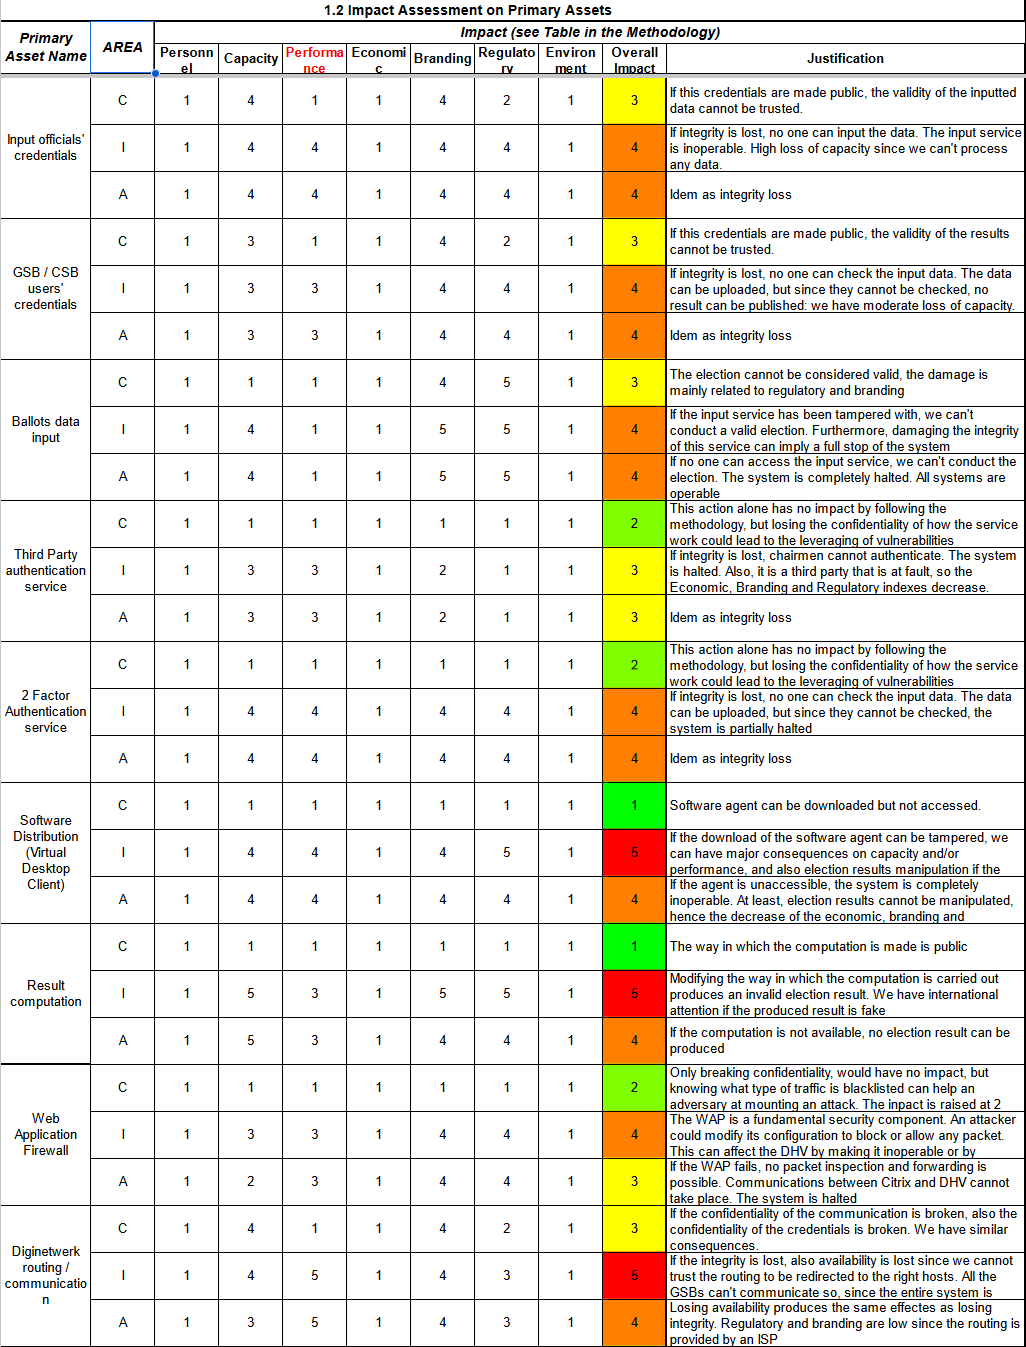
\includegraphics[keepaspectratio,width=1\textwidth]{03-risk-analysis/002-SAIV/img/cut1Impa.png}
    \label{fig:impact1}
\end{figure}

\begin{figure}[h!]
    \centering
    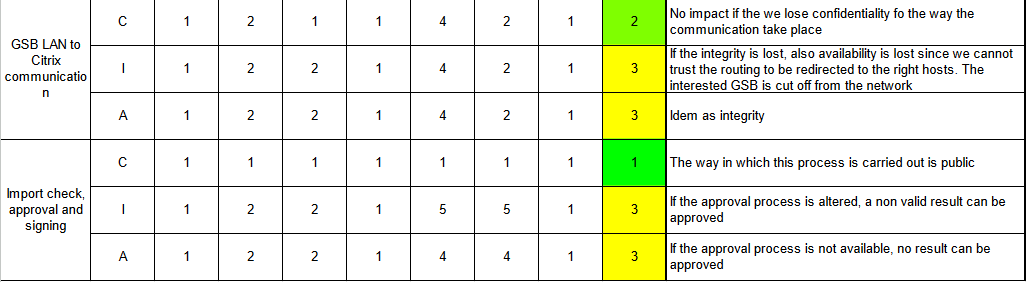
\includegraphics[keepaspectratio,width=1\textwidth]{03-risk-analysis/002-SAIV/img/cut2Impa.png}
    \caption{Impact table}
    \label{fig:impact2}
\end{figure}

\begin{figure}[h!]
    \centering
    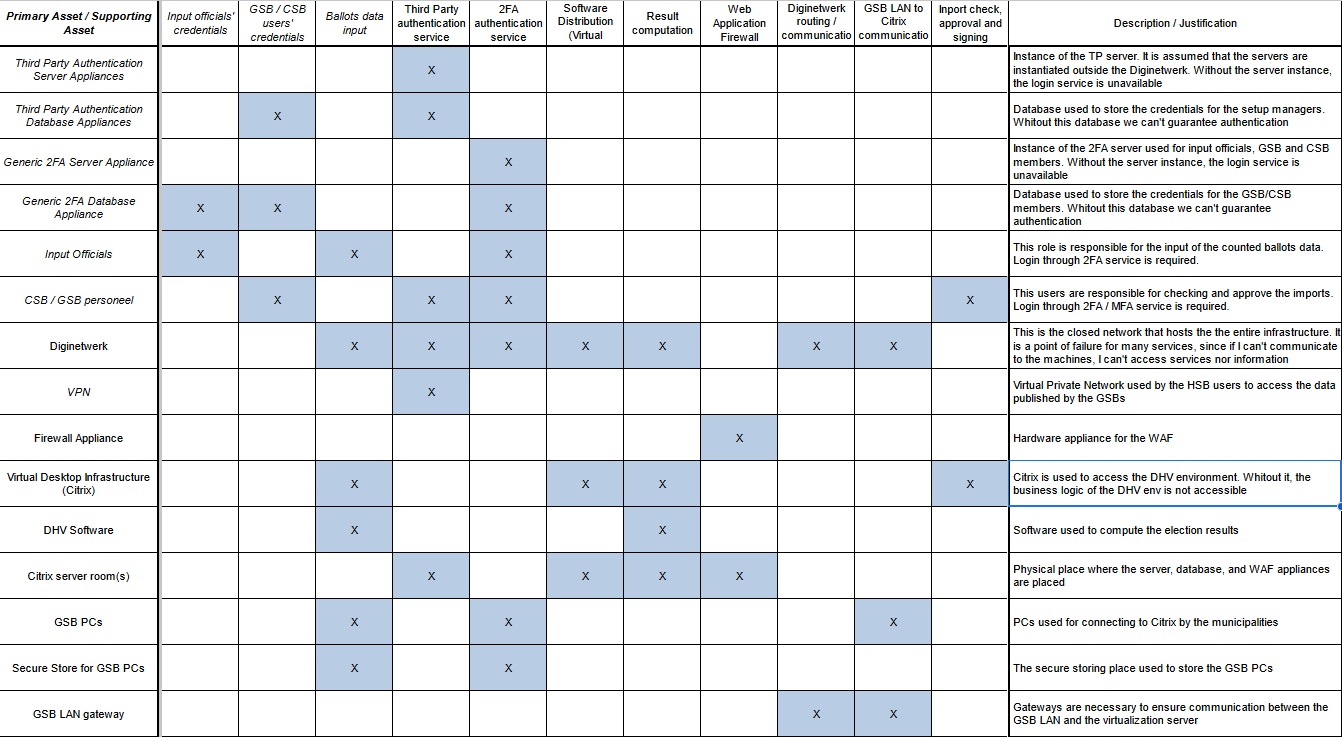
\includegraphics[keepaspectratio,width=1\textwidth]{03-risk-analysis/002-SAIV/img/linkage.png}
    \caption{Linkage table}
    \label{fig:linkage}
\end{figure}

\newpage
